\chapter{Courbes paramétrées}
La trajectoire d'un corps dans un plan est déterminé par le couple de coordonnées $(x,y)$ dépendant du temps $t$, c'est une équation paramétrique.
\begin{defi}
Soient $f$ et $g$ deux fonctions définies sur $I\subseteq
\mathbb{R}$.\\
Le point $M(t)$ de coordonnées $(f(t),g(t))$ décrit une courbe du plan $C$ appelée courbe paramétrée (de paramètre $t$).
La fonction de $I$ sur $(C)$ qui à $t$ associe $M(t)$ est un paramétrage de $(C)$.\\
Les équations $\begin{cases}x=f(t)\\y=g(t)\end{cases}$ définissent une représentation paramétrique de $\mathscr{C}$.\\
Notations : $(x=x(t),y=y(t))$ ou $t\mapsto(x(t),y(t))$
\end{defi}
Nous étudierons les propriétés des courbes paramétrées, qui peuvent être de deux natures :
\begin{itemize}
    \item Cinématique : dépendantes du paramètre $t$.\\
    ex : vitesse, accélération, ...
    \item Géométrique : indépendante du paramètre $t$.\\
    ex : tangentes, ...
\end{itemize}
\begin{rmq}
Par convention, on nomme le paramètre $t$ le temps, bien que ce dernier peut n'avoir aucun rapport avec ce dernier.\\
De même, les vecteurs correspondants aux dérivées première et seconde, sont appelés respectivement vitesse et accélération.
\end{rmq}
\section{Paramétrage et représentation graphique}
La paramétrisation d'une courbe n'est jamais unique et il est possible de passer d'un paramétrage a l'autre.
\section{Étude analytique d'une courbe paramétrée}
\subsection{Domaine de définition et intervalle d'étude}
\begin{defi}
Le domaine de définition $I$ du paramétrage est l'intersection des domaines de définition des fonctions $x(t)$ et $y(t)$.
$$\mathscr{D}_\mathscr{C}=\mathscr{D}_x\cap\mathscr{D}_y$$
\end{defi}
Une fois le domaine de définition déterminée, on cherche à réduire le domaine de définition à un intervalle d'étude afin de simplifier l'étude.
Pour ce faire, on utilise les propriétés de périodicité et de parités.
\begin{prop}
Soit la courbe $\mathscr{C}$ défini par $(x(t),y(t))$.On étudie la périodicité des deux coordonnées.\\
La coordonnée $x(t)$ est périodique si $x(t+T_1)=x(t)$ et la coordonnée $y(t)$ est périodique si $y(t+T_2)=y(t)$.\\
\newline
Si $T_1=T_2=T$ la période commune est $T$.\\
Si $T_1\neq T_2$ alors il faut déterminer la période commune $T$.\\
Pour ce faire, on a $T=\text{PPCM}(T_1,T_2)$.\\
La réduction de l'intervalle pour une courbe périodique de période $T$ est $[a,a+T]$ avec $a=0$ ou $a=\frac{T}{2}$.
\end{prop}
On rappelle que les fonctions sinus et cosinus sont $2\pi$ périodique, et la tangente est $\pi$ périodique.\\
Dans la plupart des cas, on fait en sorte que $0$ soit dans l'intervalle pour pouvoir exploiter les propriétés de symétries.
\begin{prop}
Soit la courbe $\mathscr{C}$ défini par $(x(t),y(t))$.\\
On étudie les propriétés de parités de chacune des coordonnées.
\begin{itemize}
    \item Si $x$ et $y$ sont impaires, pour tout $t$ la courbe est symétrique par rapport au centre $O$.
    \item Si $x$ est impaire et $y$ est paire, pour tout $t$ la courbe est symétrique par rapport à l'axe $(O_y)$.
    \item Si $x$ est paire et $y$ est impaire, pour tout $t$ la courbe est symétrique par rapport à l'axe $(O_x)$
    \item Si $x$ et $y$ sont paires, pour tout $t$ la courbe revient sur ces pas.
\end{itemize}
\end{prop}
\begin{ex}
On se donne un courbe $\mathscr{C}$ défini par  :
$$\begin{array}{cccc}
    \mathscr{C} \ : & \mathscr{D}_{\mathscr{C}} & \to & \mathbb{R} \\
         & t & \mapsto & \begin{cases}x(t)=\sin(\frac{3t}{2})\\y(t)=\sin(\frac{t}{3})\end{cases}
\end{array}$$
On recherche la période de chaque coordonnées :
\begin{align*}
    & x(t+T)=x(t)\\
    \Leftrightarrow & \sin\left(\frac{3t}{2}+T\right)=\sin\left(\frac{3t}{2}\right) \\
    \Leftrightarrow & \sin\left(3t+4\pi\right)\\
    \Leftrightarrow & \sin\left(t+\frac{4\pi}{3}\right)
\end{align*}
On déduit donc que la période de $x(t)$ est $T=\frac{4\pi}{3}$.
\begin{align*}
    & y(t+T)=y(t)\\
    \Leftrightarrow & \sin\left(\frac{t}{3}+2\pi\right) \\
    \Leftrightarrow & \sin\left(t+6\pi\right)
\end{align*}
On déduit donc que la période de $y(t)$ est $T=6\pi$.\\
On cherche maintenant la période commune : en cherchant $PPCM(4,6)$.
On obtient une période commune $T=12\pi$
\end{ex}
\subsection{Étude des branches infinies}
Une fois l'intervalle d'étude déterminé, on se concentre sur l'étude des branches infinies.
\begin{defi}
Soit une courbe $\mathscr{C}$ défini par ses coordonnées $(x(t),y(t))$ sur son domaine de définition $\mathscr{D}_\mathscr{C}$. On que dit que la courbe $\mathscr{C}$ possède une branche infinie si au moins l'une des quantités suivantes : $a$, $l$ ou $m$ tend vers l'infini.\\
$$\lim\limits_{t\to a}\mathscr{C}=\begin{cases}\lim\limits_{t\to a}x(t)=l\\\lim\limits_{t\to a}y(t)=m\end{cases}$$
\end{defi}
La définition ci-dessus, nous indique l'existence de branches infinies.\\
Mais il faut maintenant déterminer si la courbe $\mathscr{C}$ possède des asymptotes ou des branches paraboliques.\\
Cette information nous permet de tracer les courbes plus facilement.
\begin{prop}
Soit une courbe $\mathscr{C}$ défini par ses coordonnées $(x(t),y(t))$ sur son domaine de définition $\mathscr{D}_\mathscr{C}$.On détermine la nature des branches infinies ainsi que son équation, en suivant les critères ci-après :
\begin{itemize}
    \item Si $\lim\limits_{t\to a}x(t)=\pm\infty$ et $\lim\limits_{t\to a}y(t)=y_0$ avec $y_0\in\mathbb{R}$, la courbe admet une asymptote horizontale d'équation $y=y_0$.
    \item Si $\lim\limits_{t\to a}x(t)=x_0$ et $\lim\limits_{t\to a}y(t)=\pm\infty$ avec $x_0\in\mathbb{R}$, la courbe admet un asymptote verticale d'équation $x=x_0$
    \item Si $\lim\limits_{t\to a}x(t)=\pm\infty$ et $\lim\limits_{t\to a}y(t)=\pm\infty$, alors possible asymptote ou branche parabolique :
    \begin{itemize}
        \item Si $\lim\limits_{t\to a}\frac{y(t)}{x(t)}=\pm\infty$, la courbe admet une branche parabolique de direction asymptotique $O_y$
        \item Si $\lim\limits_{t\to a}\frac{y(t)}{x(t)}=0$, la courbe admet une branche parabolique de direction asymptotique $O_x$
        \item Si $\lim\limits_{t\to a}\frac{y(t)}{x(t)}=a$, il faut continuer l'étude :
        \begin{itemize}
            \item Si $\lim\limits_{t\to a} y(t)-ax(t)=\pm\infty$, la courbe admet une branche parabolique de direction asymptotique $y=ax$.
            \item Si $\lim\limits_{t\to a} y(t)-ax(t)=b$ avec $b\in\mathbb{R}$, la courbe admet une asymptote oblique d'équation $y=ax+b$
        \end{itemize}
    \end{itemize}
\end{itemize}
\end{prop}
SChéma et exemples
\subsection{Étude locale et points singuliers}
On commence dans un premier temps par  définir le vecteur $\overrightarrow{OM(t)}$ (autrement appelé $\overrightarrow{M(t)}$), qui est défini par $\begin{pmatrix}x(t)\\y(t)\end{pmatrix}$.\\
Afin d'amorcer une étude locale d'une courbe paramétrée il convient de dériver ce vecteur, on a donc : $\overrightarrow{M^{\prime}(t)}=\begin{pmatrix}x^{\prime}(t)\\y^{\prime}(t)\end{pmatrix}$, on obtient le vecteur vitesse.\\
Tout comme l'étude d'une fonction, tout ce qu'il de plus classique, l'essentiel de l'étude déroule au niveau des points d'annulations de ces dérivées.
\subsubsection{Tangentes}
\begin{prop}
Soit $\mathscr{C}$ une courbe paramétrée par ses coordonnées $x(t)$ et $y(t)$.\\
Nous considérons leurs dérivées, respectivement $x^{\prime}(t)$ et $y^{\prime}(t)$.
\begin{itemize}
    \item Si $x^{\prime}(t_0)=0$ et $y^{\prime}(t_0)\neq0$, la courbe admettra une tangente verticale en $t=t_0$.
    \item Si $x^{\prime}(t_0)\neq0$ et $y^{\prime}(t_0)=0$, la courbe admettra une tangente horizontale en $t=t_0$.
\end{itemize}
\end{prop}
On peut se convaincre assez facilement de la direction des tangentes à l'aide du petit raisonnement suivant.\\
En effet, si $x^{\prime}(t_0)=0$, la dérivée est entièrement portée par le vecteur unitaire $\overrightarrow{y}$, de ce fait la tangente ne peut être que verticale, et réciproquement.
\begin{ex}
On considère la courbe $\mathscr{C}$ définie par :
$$\begin{array}{cccc}
    \mathscr{C} \ : & \mathscr{D}_{\mathscr{C}} & \to & \mathbb{R} \\
         & t & \mapsto & \begin{cases}x(t)=\frac{4t^2-1}{t^3+1}\\y(t)=\frac{4t^3-t}{t^3+1}\end{cases}
\end{array}$$
\begin{minipage}{0.6\linewidth}
On dérive la composante $x(t)$ :
$$x^{\prime}(t)=\frac{x(-4x^3+3x+8)}{(t^3+1)^2}$$
On résout l'équation $x^{\prime}(t)=0$.\\
On obtient $S=\{0;1,46\}$\\
La courbe admet deux tangentes verticales.\\
\\
On dérive la composante $y(t)$ :
$$y^{\prime}(t)=\frac{2t^3+12t^2-1}{(t^3+1)^2}$$
On résout l'équation $y^{\prime}(t)=0$.\\
On obtient  $S=\left\{-5,99 ; -0,3; 0,28 \right\}$ .\\
La courbe admet trois tangentes horizontales.

\end{minipage}
\begin{minipage}{0.4\linewidth}
\begin{pspicture*}(-3, -3)(3,5)
\psgrid[subgriddiv=0,griddots=10,gridlabels=7pt,gridcolor=gray]
\parametricplot[plotstyle=curve,algebraic,linecolor=red]{-5}{5}{(4*t^2-1)/(t^3+1) | (4*t^3-t)/(t^3+1) }
\psaxes[ticks=none,labels=none]{->}(0,0)(-3,-3)(3,5)
\end{pspicture*}
\end{minipage}
\end{ex}

\subsubsection{Points réguliers et singuliers}
\begin{defi}
Soit $\mathscr{C}$ une courbe paramétrée par ses coordonnées $x(t)$ et $y(t)$.
Nous considérons le vecteur vitesse $\overrightarrow{v(t)}$ du point $M(t)$.
\begin{itemize}
    \item Si $v(t_0)\neq\overrightarrow{0}$ alors la courbe admet en $t=t_0$ un point régulier.\\
    \item Si $v(t_0)=\overrightarrow{0}$ alors la courbe admet en $t=t_0$ un point singulier.
\end{itemize}
\end{defi}
Il est nécessaire de bien comprendre ce que sont ces deux points.
Un point régulier est "un point normal de la courbe", c'est à dire que la courbe est tangente au vecteur vitesse $\overrightarrow{v(t)}$.\\
Un point singuliers quant à lui est un point très particulier qui peut être de plusieurs natures.
Néanmoins, son étude locale est, par définition, impossible en se cantonnant uniquement au vecteur vitesse.
\\
\\
Pour remédier à cela, on va faire un développement limité en $t_0$, au minimum à l'ordre 3.
On rappel la formule de Taylor, pour une fonction $f$ en un point $x_0$ à l'ordre $n$ : $$P_n(x)=\sum_{i=1}^{n}f^{(i)}(x_0)\frac{(x-x_0)^{i}}{i!}$$
On calcul les développements limités des deux coordonnées.
$$x(t)=x(t_0)+v_x(t_0)(t-t_0)+x^{\prime\prime}(t_0)\frac{(t-t_0)^2}{2!}+x^{(3)}(t_0)\frac{(t-t_0)^3}{3!}+...+o((t-t_0)^n)$$
et
$$y(t)=y(t_0)+v_y(t_0)(t-t_0)+y^{\prime\prime}(t_0)\frac{(t-t_0)^2}{2!}+y^{(3)}(t_0)\frac{(t-t_0)^3}{3!}+...+o((t-t_0)^n)$$
Puis on rassemble ces deux développement limités en un vecteur :
$$\overrightarrow{M(t)}=\begin{pmatrix}x(t_0)\\y(t_0\end{pmatrix}+\begin{pmatrix}v_x(t_0)\\v_y(t_0)\end{pmatrix}(t-t_0)+\begin{pmatrix}x^{\prime\prime}(t_0)\\y^{\prime\prime}(t_0)\end{pmatrix}\frac{(t-t_0)^2}{2}+\begin{pmatrix}x^{(3)}(t_0)\\y^{(3)}(t_0)\end{pmatrix}\frac{(t-t_0)^3}{6}+...+o(\|\overrightarrow{M(t)}\|^n)$$
Or par définition d'un point singulier ($\overrightarrow{v(t_0)}=\overrightarrow{0}$), on a :
$$\overrightarrow{M(t)}=\begin{pmatrix}x(t_0)\\y(t_0)\end{pmatrix}+\begin{pmatrix}x^{\prime\prime}(t_0)\\y^{\prime\prime}(t_0)\end{pmatrix}\frac{(t-t_0)^2}{2}+\begin{pmatrix}x^{(3)}(t_0)\\y^{(3)}(t_0)\end{pmatrix}\frac{(t-t_0)^3}{6}+...+o(\|\overrightarrow{M(t)}\|^n)$$
Une fois cela fait nous cherchons les deux premiers vecteurs (associées a des degrés supérieurs à $2$ dans le développement limité), non colinéaires.
Ces deux vecteurs nous permettrons de définir la nature du point singulier, ainsi que le sens de parcours de la courbe à travers celui-ci.

\begin{prop}
Soit une courbe $\mathscr{C}$ ayant un point singulier au point $t=t_0$.\\
Le développement limité de la courbe $\mathscr{C}$ au point $t=t_0$ à l'ordre $n$ est le suivant :
$$\overrightarrow{M(t)}=\begin{pmatrix}x(t_0)\\y(t_0)\end{pmatrix}+...+\underbrace{\begin{pmatrix}x^{(p)}(t_0)\\y^{(p)}(t_0)\end{pmatrix}}_{\overrightarrow{l}}\frac{(t-t_0)^p}{p!}+...+\underbrace{\begin{pmatrix}x^{(q)}(t_0)\\y^{(q)}(t_0)\end{pmatrix}}_{\overrightarrow{m}}\frac{(t-t_0)^q}{q!}+...+o(\|\overrightarrow{M(t)}\|^n)$$
Avec les vecteurs $\overrightarrow{l}$ et $\overrightarrow{m}$, les deux premiers vecteurs non colinéaires.\\
La nature du point singulier est donnée par les critères suivants :
\begin{itemize}
    \item Si $p$ est impair et $q$ est pair, alors il s'agit d'un point régulier.
    \item Si $p$ est impair et $q$ est impair, alors il s'agit d'un point d'inflexion.
    \item Si $p$ est pair et $q$ est impair, alors il s'agit d'un point de rebroussement de $1^{\text{ère}}$ espèce.
    \item Si $p$ est pair et $q$ est pair, alors il s'agit d'un point de rebroussement de $2^{\text{nde}}$ espèce.
\end{itemize}
\end{prop}
propriétés sur le sens de parcours demander à la prof

Images à faires

\subsubsection{Convexité}
Dans le cas d'un point d'inflexion, il peut-être utile de chercher si avant et après lui la courbe est convexe ou concave.
\subsection{Tableau de variation}
\subsection{Applications}
\begin{meth}
Soit une courbe $\mathscr{C}$, voici le déroulement de son étude :
\begin{enumerate}
    \item Détermination de son ensemble de définition
    \item Étude de la périodicité et des symétries pour un éventuelle réduction de l'intervalle d'étude.
    \item Étude des limites et des branches infinies, déterminer les asymptotes.
    \item Étude locale, recherche des tangentes et des possibles points de rebroussements et d'inflexion.
    \item Dressage du tableau de variation.
    \item Dessin de la courbe $\mathscr{C}$.
\end{enumerate}
\end{meth}
\begin{ex}

On considère la courbe $\mathscr{C}$ définie par :
$$\begin{array}{cccc}
    \mathscr{C} \ : & \mathscr{D}_{\mathscr{C}} & \to & \mathbb{R} \\
         & t & \mapsto & \begin{cases}\displaystyle x(t)=\frac{2t}{1+t^2}\\\displaystyle y(t)=\frac{2+t^3}{1+t^2}\end{cases}
\end{array}$$
On commence dans un premier temps par définir l'ensemble de définition.
Dans notre cas, le dénominateur est commun aux deux fonctions.\\
On cherche les valeurs interdites du dénominateur:
\begin{align*}
    & 1+t^2=0\\
    \Leftrightarrow & t^2=-1\\
    \Leftrightarrow & S=\{\varnothing\}
\end{align*}
En effet, une racine carrée ne pouvant être négative dans $\mathbb{R}$, les fonctions n'admettent aucune valeur interdite.
On obtient : $\mathscr{D}_\mathscr{C}=\mathbb{R}$.\\
On recherche ensuite d'éventuelles propriétés de périodicité et de parité.\\
Ici il n'y a pas de périodicité car il n'y aucune fonction trigonométrique.\\
On pose ensuite :
\begin{align*}
& x(-t)=\frac{2(-t)}{1+(-t)^2}=\frac{-2t}{1+t^2}=-x(t)\\
& y(-t)=\frac{2+(-t)^3}{1+(-t)^2}=\frac{2-t^3}{1+t^2}
\end{align*}
On déduit que la coordonnée $x(t)$ est impaire et $y(t)$ est ni paire ni impaire.\\
Donc la courbe n'admet aucune parité et donc aucune symétrie.\\

On entame donc l'étude des branches infinies de la courbe.\\
On cherche les limites en $+\infty$ et $-\infty$ de la courbe $\mathscr{C}$:\\
${\displaystyle \lim_{t\to +\infty}}x(t)=\frac{2t}{t^2\left(\frac{1}{t^2}+1\right)}=\frac{2}{t\left(\frac{1}{t^2}+1\right)}=0^{+}$\\
$\displaystyle\lim_{t\to-\infty}x(t)=\frac{2}{t\left(\frac{1}{t^2}+1\right)}=0^{-}$\\
$\displaystyle\lim_{t\to +\infty}y(t)=\frac{2+t^3}{1+t^2}=\frac{t^3\left(\frac{2}{t^3}+1\right)}{t\left(\frac{1}{t^2}+1\right)}=\frac{t^2\left(\frac{2}{t^3}+1\right)}{\frac{1}{t^2}+1}=+\infty$\\
$\displaystyle\lim_{t\to -\infty}y(t)=\frac{t^2\left(\frac{2}{t^3}+1\right)}{\frac{1}{t^2}+1}=-\infty$\\
La courbe n'admet aucune asymptote.\\

On passe désormais à l'étude local de la courbe $C$.
On détermine le vecteur vitesse :\\
$$\overrightarrow{v}=\begin{pmatrix}x^{\prime}\\y^{\prime}\end{pmatrix}=\begin{pmatrix}\frac{-2t+2}{(1+t^2)^2}\\\frac{t(t^3+3t-4)}{(1+t^2)^2}\end{pmatrix}$$
On cherche les points d'annulation des dérivées :
\begin{align*}
    \Leftrightarrow & \frac{-2t+2}{(1+t^2)^2}=0\\
    \Leftrightarrow & -2t+2=0\\
    \Rightarrow & S=\{1\}
\end{align*}
\begin{align*}
    \Leftrightarrow & \frac{t(t^3+3t-4)}{(1+t^2)^2}\\
    \Leftrightarrow & t(t^3+3t-4)=0\\
    \Leftrightarrow & t(t-1)(t^2+t-4)=0\\
    \Rightarrow & S=\{0,1\}
\end{align*}
On voit que pour $t=1$, la courbe admet un possible point singulier et une tangente horizontale pour $t=0$.\\
Pour plus de détails, on effectue un développement limité du vecteur $\overrightarrow{v}$ au point 1 à l'ordre 5.
On pose $t=h+1$. On peut donc réécrire :
$$\begin{cases}\displaystyle x(h)=\frac{2(h+1)}{1+(1+h)^2}=(2h+2)\frac{1}{2+2h+h^2}=(2h+2)\frac{1}{2}\times\frac{1}{1+h+\frac{h^2}{2}}\\
\displaystyle y(h)=\frac{2+(h+1)^3}{1+(1+h)^2}=(h^3+3h^2+3h+3)\frac{1}{2}\times\frac{1}{1+h+\frac{h^2}{2}}\end{cases}$$
On pose $u=h+\frac{h^2}{2}$, on cherche le développement limité de $\frac{1}{1+u}$.
$$\displaystyle\frac{1}{1+u}=\sum_{k=0}^n(-1)^ku^k+o(x^n)$$
A l'ordre 5, on a donc :  
\begin{align*}
    \frac{1}{1+u}&=1-u+u^2-u^3+u^4-u^5+o(u^5)\\
     &=1-\left(h+\frac{h^2}{2}\right)+\left(h+\frac{h^2}{2}\right)^2-\left(h+\frac{h^2}{2}\right)^3+\left(h+\frac{h^2}{2}\right)^4-\left(h+\frac{h^2}{2}\right)^5+o(h^5)\\
     &=1-h-\frac{h^2}{2}+\left(h^2+h^3+\frac{h^4}{2}\right)-\left(h^3+\frac{3h^4}{2}+h^5\right)+\left(h^4+\frac{6h^5}{2}\right)+o(h^5)\\
     &=1-h+\left(\frac{-1}{2}+1\right)h^2+\left(\frac{1}{2}-\frac{3}{2}+1\right)h^4+\left(-1+\frac{6}{2}\right)h^5+o(h^5)\\
     &=1-h+\frac{h^2}{2}+\frac{4}{6}h^5+o(h^5)=\frac{1}{1+h+\frac{h^2}{2}}\\
\end{align*}
Pour déterminer les développements limités de chacune des composantes, il nous suffit de poser :
\begin{align*}
    x(h)&=(h+1)\frac{1}{1+h+\frac{h^2}{2}}\\
    &=(h+1)\left(1-h+\frac{h^2}{2}+\frac{4}{6}h^5+o(h^5)\right)\\
    &=h-h^2+\frac{h^3}{2}+1-h+\frac{h^2}{2}+\frac{4}{6}h^5+o(h^5)\\
    &=1+\left(-1+\frac{1}{2}\right)h^2+\frac{h^3}{2}+\frac{2}{3}h^5+o(h^5)\\
    &=1-\frac{h^2}{2}+\frac{h^3}{2}+\frac{2}{3}h^5+o(h^5)
\end{align*}
\begin{align*}
    y(h)&=\frac{1}{2}\left(h^3+3h^2+3h+3\right)\frac{1}{1+h+\frac{h^2}{2}}\\
    &=\frac{1}{2}\left(h^3+3h^2+3h+3\right)\left(1-h+\frac{h^2}{2}+\frac{2}{3}h^5+o(h^5)\right)\\
    &=\frac{1}{2}\left(h^3-h^4+\frac{h^5}{2}+3h^2-3h^3+\frac{3}{2}h^4+3h-3h^2+\frac{3}{2}h^3+3-3h+\frac{3}{2}h^2+2h^5+o(h^5)\right)\\
    &=\frac{1}{2}\left(3+\left(3-3+\frac{3}{2}\right)h^2+\left(1-3+\frac{3}{2}\right)h^3+\left(-1+\frac{3}{2}\right)h^4+\left(\frac{1}{2}+\frac{3}{2}+2\right)h^5+o(h^5)\right)\\
    &=\frac{1}{2}\left(3+\frac{3}{2}h^2-\frac{h^3}{2}+\frac{h^4}{2}+4h^5+o(h^5)\right)\\
    &=\frac{3}{2}+\frac{3}{4}h^2-\frac{h^3}{4}+\frac{h^4}{4}+2h^5+o(h^5)
\end{align*}
On effectue le changement de variable inverse sur $h$ sur les deux coordonnées, on obtient alors :
$$x(t)=1-\frac{(t-1)^2}{2}+\frac{(t-1)^3}{2}+\frac{2}{3}(t-1)^5+o((t-1)^5)$$
$$y(t)=\frac{3}{2}+\frac{3}{4}(t-1)^2-\frac{(t-1)^3}{4}+\frac{(t-1)^4}{4}+2(t-1)^5+o((t-1)^5)$$
On peut construire le vecteur position à partir des développements limités :

$$\overrightarrow{M}(t)=\begin{pmatrix}1\\\frac{3}{2}\end{pmatrix}+\begin{pmatrix}-\frac{1}{2}\\\frac{3}{4}\end{pmatrix}(t-1)^2+\begin{pmatrix}\frac{1}{2}\\\frac{-1}{4}\end{pmatrix}(t-1)^3+\begin{pmatrix}0\\\frac{1}{4}\end{pmatrix}(t-1)^4+\begin{pmatrix}\frac{2}{3}\\2\end{pmatrix}(t-1)^5+o(\|\overrightarrow{M}(t)\|^5)$$
Ici les deux premier vecteurs non colinéaires sont portées par les puissance $p=2$ et $q=3$.
$p$ est paire et $q$ est impaire, on voit que le point $\left(1,\frac{3}{2}\right)$ est un point de rebroussement de $1^{\text{ère}}$ espèce.\\
Les vecteurs $\overrightarrow{u}=\begin{pmatrix}\frac{-1}{2}\\\frac{3}{4}\end{pmatrix}$ et $\overrightarrow{v}=\begin{pmatrix}\frac{1}{2}\\\frac{-1}{4}\end{pmatrix}$ forment une base.\\
On compile toutes les informations précédemment déterminées dans un tableau de variation.
\begin{center}
\begin{tikzpicture}
\tkzTabInit{$t$ /1,$x^{\prime}$ / 1 , $x(t)$ / 2  , $y^{\prime}$ / 1 , $y(t)$ / 2}{$-\infty$,0,1,$+\infty$}
\tkzTabLine{,,+,,z,-}
\tkzTabVar{-/ $0^{+}$,+/ $0$,+/ $1$,-/ $0$}
\tkzTabLine{+,,z,-,z,+}
\tkzTabVar{-/$-\infty$,+/ $2$, -/ $\frac{3}{2}$,+/ $+\infty$}
\end{tikzpicture}
\end{center}
Il ne nous reste plus qu'a tracer la courbe $\mathscr{C}$.
\begin{center}
\begin{pspicture*}(-3, -4)(3,5)
\psgrid[subgriddiv=0,griddots=10,gridlabels=7pt,gridcolor=gray]
\parametricplot[plotstyle=curve,algebraic,linecolor=red]{-5}{5}{2*t/(1+t^2) | (2+t^3)/(1+t^2) }
\psaxes[ticks=none,labels=none]{->}(0,0)(-3,-4)(3,5)
\end{pspicture*}
\end{center}
\end{ex}
\section{Courbes en polaire}
Cette section se concentrera sur l'étude des fonctions défini
\begin{defi}
Une courbe en polaire est une courbe paramétrée par :
$$\begin{array}{cccc}
    \mathscr{C} \ : & \mathscr{D}_{f} & \to & \mathbb{R} \\
         & \theta & \mapsto & r(\theta)
\end{array}$$
où $r(\theta)$ est la distance algébrique du point $M$ à l'origine.\\
Autrement dit, $\overrightarrow{OM(\theta)}=r(\theta)\overrightarrow{u_r(\theta)}=r(\theta)\begin{pmatrix}\cos\theta\\\sin\theta\end{pmatrix}$
\end{defi}
Le fait que $r(\theta)$ soit une distance algébrique traduit le fait que ...\\
Le point $M(\theta)$ est donc bien à une distance $|r(\theta)|$ mais dans la direction $-\overrightarrow{u_r(\theta)}$.
\begin{prop}
Soit $\mathscr{C}$ une courbe en polaire, un paramétrage de la courbe $\mathscr{C}$ serait :
$$r(\theta)\Leftrightarrow\begin{cases}x(\theta)=r(\theta)\cos(\theta)\\y(\theta)=r(\theta)\sin(\theta)\end{cases}$$
\end{prop}
La plupart du temps, ramener une courbe en polaire en paramétrée n'est pas un choix judicieux pour son étude.
\subsection{Domaine de définition et intervalle d'étude}
Périodicité :
Si la période n'est pas multiple de $2\pi$, alors il faut faire des rotations pour déterminer la courbe dans son ensemble.
Symétries :

\subsection{Étude des branches infinies}

\begin{prop}
\begin{itemize}
    \item Si $r(\theta)$ est périodique :
    \begin{itemize}
        \item Si $\lim\limits_{\theta\to \theta_0}r(\theta)\sin{\theta-\theta_0}=l$ avec $l\in\mathbb{R}$, la courbe admet une asymptote oblique d'équation $y=l$ dans le repère tourné d'angle $\theta_0$.
    \end{itemize}
    \item Si $r(\theta)$ n'est pas périodique :
    \begin{itemize}
        \item Si $\lim\limits_{\theta\to\pm\infty}r(\theta)=\pm\infty$, la courbe tend vers l'infini en spiralant.
        \item Si $\lim\limits_{\theta\to\pm\infty}r(\theta)=0$, la courbe tend vers $0$ en spiralant.
        \item Si $\lim\limits_{\theta\to\pm\infty}r(\theta)=l$ avec $l\in\mathbb{R}^{*}$, la courbe s'enroule vers le cercle centré à l'origine et de rayon $|l|$.
    \end{itemize}
\end{itemize}
\end{prop}
\subsection{Étude locale}
\subsection{Tableau de variation}
\subsection{Applications}
\begin{ex}
Soit la courbe $\mathscr{C}$ défini par la fonction $r(\theta)$:
$$\begin{array}{ccccc}
    r(\theta) & : & \mathscr{D}_r & \to & \mathbb{R} \\
     & & \theta & \mapsto & 1+\frac{1}{\theta - \frac{\pi}{4}}
\end{array}$$
\end{ex}
\section{Coniques}